%!TEX root = ../../main.tex

\chapter{Grundlagen}
\label{chapter:3}

Bevor mit der eigentlichen Arbeit der Studienarbeit begonnen wird, sollten wichtige Grundstrukturen geklärt werden. Das folgende Kapitel stellt die wichtigsten Grundstrukturen und Prinzipien vor, die im Laufe dieser Studienarbeit relevant werden. Es werden Konzepte zur Erstellung und Umsetzung der Umfrage sowie zu Programmiertechnologien geboten.

\section{Humanzentriertes Design}

Beim Entwickeln neuer Software setzen erfahrene SoftwareentwicklerInnen häufig auf einen gut durchdachten Plan und Struktur. Dabei wird auf bestimmte Entwicklungsprozesse gesetzt. Einer der bekanntesten Prozesse in der Softwareentwicklung ist hierbei der “\acf{SDLC}” (kurz: \acs{SDLC}). Der \acs{SDLC} wird genutzt, um möglichst effiziente, kostengünstige Software mit hoher Qualität zu designen, entwickeln und zu produzieren.\cite{shylesh:2017} Es gibt eine Menge verschiedene Modelle des \acs{SDLC}, jedoch haben alle Modelle im Grunde dieselbe Struktur: Planen - Design - Implementieren - Testen. Besonders auf den Aspekt "Design" wird in diesem Kapitel genauer eingegangen.

Eine der weitverbreitetsten Designmodelle ist das “\acf{HCD}” (kurz: \acs{HCD}, dt.: menschenzentriertes Design). Dabei handelt es sich um eine Designtechnik, bei der der Mensch im Vordergrund des Entwicklungsprozesses steht. Laut der Webseite der Harvard Business School liegen die Ziele des \acs{HCD} darin, die Ziele, Wünsche und Vorlieben des Produktnutzers stetig im Auge zu behalten. Dort beschreibt ein Dekan der Harvard Business School vier grundlegende Phasen im \acs{HCD}. Diese sind laut Dekan Srikant Datar folgende Phasen: Clarify - Ideate - Develop - Implement. Wiederum definiert Sim van der Ryn in seinem Paper \"Human Centered Design\" aus dem Jahr 2013 das Vorgehen des \acs{HCD} ein wenig anders, jedoch ähnlich. Dieser schreibt, dass man sich zuerst mit den potenziellen NutzerInnen beschäftigen sollte. Anschließend wird das Problem definiert, eine Idee erarbeitet, ein Prototyp erstellt und abschließend getestet.\cite{vanderryn:2013, hbsc:2020}

\begin{figure}[h]
    \centering
    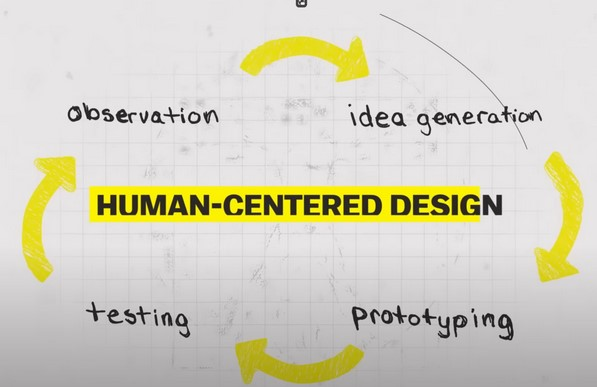
\includegraphics[width=1\textwidth]{images/03/HCD.jpg}
    \caption{Humand Centered Design Prozess}
\end{figure}

Zu den Vorteilen des \acs{HCD} gehört unter anderem eine hohe Nutzerzufriedenheit, da die Meinung der Personen direkten Einfluss auf das Design des Produkts hat und somit sichergestellt wird, dass alle Bedürfnisse und Erwartungen an das Produkt erfüllt werden \cite{hcd:2021}. Zudem kann dadurch die Wechselwirkung zwischen Menschen und Objekten besser verstanden werden, da man durch die Designfrage wichtige Erkenntnisse über das Verhalten bzw. Bedürfnisse der Menschen oder zumindest einer Personengruppe bekommt. \cite{let:2022}

Zu den Vorteilen des \acs{HCD} gehören unter anderem eine hohe Nutzerzufriedenheit, da die Meinung von Personen unmittelbaren Einfluss auf das Design des Produkts nimmt und so sicherstellt, dass alle Bedürfnisse und Erwartungen an das Produkt garantiert werden.\cite{hcd:2021} Zudem kann dadurch die Wechselwirkung zwischen Menschen und Objekten besser verstanden werden, da man durch die Designfrage wichtige Erkenntnisse über das Verhalten bzw. die Bedürfnisse der Menschen oder zumindest einer Personengruppe bekommt.\cite{let:2022}

Allerdings gibt es auch einige Nachteile bzw. Probleme des \acs{HCD}. Ein Aspekt wäre der rapide Produktlebenszyklus. Durch die ständig wechselnden Bedürfnisse und Anforderungen an ein Produkt stehen DesignerInnen und Designteams ständig unter großen Herausforderungen, um die Ansprüche treffen zu können. Häufig könnten aber auch eben diese menschlichen Anforderungen an ein Produkt zum Problem werden, da diese Anforderungen nicht umsetzbar und realisierbar sind.\cite{pod:2016}

\section{Nutzerzentriertes Design}

Wenn man sich beim Entwickeln neuer Software besonders auf die NutzerInnen konzentriert und diese nach ihren Wünschen und Anregungen gestaltet, spricht man von \"User-Centered Design\" (\acs{UCD}). Ein wesentlicher Unterschied zum Humanzentrierten Design (\acs{HCD}) besteht darin, dass das Nutzerzentrierte Design soziale und kulturelle Aspekte nicht in das Design einfließen lässt. \cite{hcd2:2021} Diese Aspekte spielen beim Humanzentrierten Design eine wesentliche Rolle. Dennoch wird \acs{UCD} heutzutage oft mit \acs{HCD} gleichgesetzt. \cite{ucd1:2011}



Ein zentraler Aspekt des \acs{UCD} sind sogenannte Personas. Laut dem Buch "Persona Design in Participatory Agile Software Development" werden Personas häufig als Methode im \acs{UCD} genutzt, um fiktionale Charaktere zu erschaffen, die verschiedene NutzerInnengruppen repräsentieren. \cite{personaDesign:2020} Eine Persona wird dabei meistens in Form einer Erzählung beschrieben. \cite{ucd1:2011} Das Ziel besteht darin, die Persona wie eine reale Person darzustellen und ihre Bedürfnisse anschaulich innerhalb einer Geschichte zu präsentieren, um sie in die Entwicklung des Produkts einzubeziehen. \cite{ucd1:2011}

Grundsätzlich beginnt eine solche Erzählung mit einer Beschreibung der Person. \cite{ucd1:2011} Während der Beschreibung werden wichtige charakteristische Merkmale der Persona wie Vorlieben, Abneigungen, Beruf usw. hervorgehoben. \cite{ucd1:2011}

\subsection{Erstellen einer Persona}
Die Erstellung einer Persona ist ein wesentlicher Bestandteil des \acs{UCD}. In einem wissenschaftlichen Paper der Universität Rostock wird der Prozess der Persona-Erstellung beschrieben. Der gesamte Entwicklungsprozess einer Persona ist in der folgenden Abbildung dargestellt:

\begin{figure}[h]
    \centering
    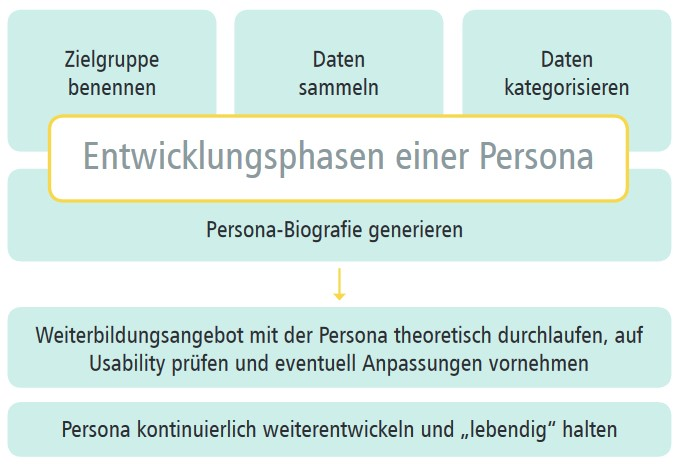
\includegraphics[width=1\textwidth]{images/03/entwicklungPersona.jpg}
    \caption{Entwicklungsprozess der Persona \cite{personamethode}}
    \label{personaEntwicklungsPhasen}
\end{figure}

Zu sehen ist, dass nahezu alle Schritte, welche vor der Erstellung von Personas passieren, mit Daten zutun haben. Besonders das Sammelen und Kategorisieren der Daten wird hier thematisiert.\cite{personamethode} Dazu schreibt der Wissenschaftler Frank Ploß in seiner Diplomarbeit \"Usability Engineering in einem Open-Source-Projekt\", welches ebenfalls von der Universität Rostock zitiert wird, dass es sich bei den eizenlenen Designstufen um ein iteratives Modell handelt.\cite{osp:masterthesis}
Das bedeutet im Grunde genommen nur, dass die einzelnen Schritte aufeinandner aufbauend sind. In dem Artikel wird zudem erwähnt, dass bereits im Vorfeld der Personaentwicklung Fragen über die Zielgruppe gestellt werden sollen, um die Erschaffung einer Persona zu vereinfachen.\cite{personamethode}
Dieser Schritt wird im Rahmen der Studienarbeit ausführlicher innerhalb einer Umfrage durchgeführt.

Nach dem Sammeln und Kategorisieren der Daten wird die Persona definiert.\cite{personamethode} In diesem Schritt wird laut dem wissenschaftlichen Artikel der Universität Rostock eine Art Kurzbiografie für jede Persona erschaffen.\cite{personamethode} Als Beispiel für eine Persona in der Praxis verwendet die Universität Rostock deshalb Steckbriefe, um ihre Personas so kurz wie möglich, mit möglichst vielen Informationen darzustellen.\cite{personamethode}

Zum Abschluss sollten die Personas noch einen so genanntes Weiterbildungsangebot durchlaufen. Das bedeutet, dass man sich beispielsweise in die Sicht eines Kunden versetzt und als die gerade eben erstellte Persona den Einkaufsprozess durchläuft.\cite{personamethode} Dieser Schritt hilft dabei, die Persona noch stärker zu definieren und evtl. Schwächen/Stärken herauszufinden.

\section{Einführung in die Webentwicklung}

Die Webentwicklung ist ein sehr großer Bereich der Softwareentwicklung und umfasst die Entwicklung von Webanwendungen, die auf den aktuellsten Technologien, Frameworks und Tools basieren. Die Schaffung zeitgemäßer Webanwendungen beinhaltet verschiedene Aspekte, von der Frontend-Entwicklung bis zur Backend-Entwicklung und der Nutzung von \acf{API}s und Datenbanken, welche alle miteinander interagieren und kommunizieren müssen.

Der Standard für die Webentwicklung ist die Verwendung von \acf{JS}, \acf{HTML} und \acf{CSS}. Diese Technologien sind die absoluten Grundlagen für die Entwicklung von Webanwendungen, auf denen alles Weitere aufbaut.

Die Frontend-Entwicklung von Webanwendungen umfasst hierbei die Verwendung von Frameworks wie \textbf{React.js}, \textbf{Angular} und \textbf{Vue}. Diese wiederum basieren auf der Programmiersprache \acl{JS} und ermöglichen die Erstellung von wiederverwendbaren Komponenten, auch bekannt als Komponentenarchitektur. Die Verwendung von Frameworks ermöglicht darüber hinaus auch die Anwendung moderner Entwicklungspraktiken wie Komponententests, Test-Driven-Development und Continuous Integration. Außerdem ermöglichen Frameworks den EntwicklerInnenn, die Entwicklungseffizienz zu verbessern und die Wartbarkeit der Anwendung zu erhöhen. Die zuvor angesprochenen Frameworks sind nur einige der vielen \acl{JS} Frameworks, die existieren. Es gibt eine Vielzahl von Frameworks, die alle ihre eigenen Stärken und Schwächen haben. Die Wahl des richtigen Frameworks hängt von den Anforderungen des Projekts ab und sollte sorgfältig abgewogen werden, um die beste Benutzererfahrung zu gewährleisten.\cite{modern-webdevelopment:1, modern-webdevelopment:2}

\subsection{Komponentenarchitektur}

Wie zuvor angesprochen ist die Komponentenarchitektur ein grundlegendes Konzept in der Webentwicklung, das darauf abzielt, die Benutzeroberfläche in wiederverwendbare und modulare Komponenten zu strukturieren. Diese Komponenten können eigenständige Teile der Benutzeroberfläche sein, die bestimmte Funktionen oder Darstellungen bereitstellen. Durch die Verwendung einer Komponentenarchitektur können EntwicklerInnen die Komplexität von Webanwendungen reduzieren, den Entwicklungsprozess beschleunigen und die Wartbarkeit verbessern.

Die Komponentenarchitektur zielt darauf ab, diverse Prinzipien zu erfüllen. In der folgenden Auflistung sind einige der wichtigsten Prinzipien aufgeführt:

\begin{itemize}
    \item \textbf{Wiederverwendbarkeit:} Komponenten können in verschiedenen Teilen einer Anwendung wiederverwendet werden, was die Entwicklung beschleunigt und den Code reduziert.
    \item \textbf{Modularität:} Die Benutzeroberfläche wird in unabhängige Komponenten aufgeteilt, die jeweils eine spezifische Aufgabe erfüllen. Diese Komponenten können dann miteinander kombiniert werden, um komplexe Benutzeroberflächen zu erstellen.
    \item \textbf{Klare Trennung von Anliegen:} Jede Komponente kann ihre eigene interne Logik und ihr eigenes Styling haben, was eine klare Trennung von Anliegen ermöglicht.
    \item \textbf{Wartbarkeit:} Die Wiederverwendbarkeit und Modularität der Komponenten erleichtern die Wartung und Aktualisierung von Anwendungen, da Änderungen an einer Komponente automatisch in allen Instanzen dieser Komponente wirksam werden.
    \item \textbf{Komposition:} Durch die Kombination mehrerer Komponenten können komplexe Benutzeroberflächen erstellt werden, die aus mehreren modularen Teilen bestehen. Diese Komposition ermöglicht es EntwicklerInnenn, die Benutzeroberfläche schrittweise aufzubauen und sie bei Bedarf zu erweitern oder anzupassen.
\end{itemize}

Diese Architektur ermöglicht es EntwicklerInnenn, die Benutzeroberfläche in kleinere, wiederverwendbare Teile zu zerlegen, die unabhängig voneinander entwickelt, getestet und gewartet werden können. Dies führt zu einer verbesserten Entwicklungseffizienz und einer höheren Codequalität, da Entwickler sich auf die Entwicklung und Wartung einzelner Komponenten konzentrieren können, anstatt sich mit der gesamten Benutzeroberfläche auseinandersetzen zu müssen.\cite{component-architecture:1, component-architecture:2}

\subsection{Programmiersprache JavaScript}
\label{chapter:3-javaScript}

\acl{JS} ist eine interpretierte Programmiersprache, welche hauptsächlich Anwendung bei Webanwendungen findet. Sie wird dafür genutzt, um Interaktionen als auch die dynamische Veränderung auf der Webseite zu ermöglichen. Dadurch kommt JavaScript größtenteils im Browser vor, also auf der Seite des Clients. JavaScript kann neben dem sehr verbreiteten objektorientierten Programmierstil auch als prozedurale Programmiersprache eingesetzt werden, dadurch ist JavaScript sehr flexibel, was einerseits vorteilhaft ist, aber auch zum Nachteil führt, da es keine konkreten Richtlinien gibt, woran man sich halten sollte. Aber JavaScript ist nicht nur im Programmierstil sehr flexibel, denn dadurch, dass es nur eine interpretierte Programmiersprache ist, besitzt es weitere Nachteile gegenüber von kompilierten Sprachen.

Einer der größten Nachteile hierbei ist, dass es bei JavaScript keine direkte Typisierung gibt, die im Vorhinein im Quellcode festgelegt wird, wie bei typisierten Programmiersprachen wie z. B. Java. Dadurch können theoretisch jegliche Art von Daten in einer Variable gespeichert werden. Das führt dazu, dass man während des Entwicklungsprozesses einfache Fehler nicht feststellen kann, sondern erst beim Ausführen der Software.
Bei Programmiersprachen, welche typisiert sind, kann dieses Problem schon im Vorhinein festgestellt werden. Dadurch können einfache Fehler wie z. B. das Datentypen nicht miteinander übereinstimmen, ob auf diese Variable in diesem Kontext zugegriffen werden kann oder dass eine Variable nicht existiert, bereits im Vorhinein festgestellt werden. Dazu kommt, dass neben den nicht typisierbaren Variablen in JavaScript die Eingabe- und Ausgabeparameter einer Funktion nicht typisieren kann. Diese Tatsache führt häufig zu Fehlern, welche erst im laufenden Betrieb der Software festgestellt werden können. Dadurch wird JavaScript-Code sehr schwer wartbar, da EntwicklerInnen beim Lesen des Quellcodes nicht genau wissen können, was in einer Variable gespeichert ist und was die Funktionen genau machen. Um den Quellcode letztlich korrekt zu verstehen, ist es nötig, sich intensiv einzuarbeiten, was sowohl viel Zeit, als auch Geld kostet.

Im Folgenden ist ein kleines Beispiel, wie sich JavaScript von Java unterscheidet hinsichtlich der Typisierung von der Deklaration von Variablen und Funktionen.

\begin{lstlisting}[caption=Java Variablen und Funktion deklarations Beispiel, label=variables-and-functions-example-java, language=Java]
    // Deklaration von Typisierten Variablen
    int name = 1;
    char name = "c";
    String name = "John";

    // Deklaration von Typisierten Funktionen
    private int add(int a, int b) {
        return a + b;
    }
\end{lstlisting}

\begin{lstlisting}[caption=JavaScript Variablen und Funktion deklarations Beispiel, label=variables-and-functions-example-javascript, language=JavaScript]
    // Deklaration von Variablen
    let a = 1;
    let b = "c";
    let c = "John";

    // Deklaration von Funktionen
    function add(a, b) {
        return a + b;
    }
\end{lstlisting}

Grundsätzlich ist es in JavaScript nicht möglich direkt zu wissen, was in einer Variable sein kann. Schon bei einfachen Funktionen wie einer Additionsfunktion wird in der JavaScript-Variante nicht direkt deutlich, dass eine Zahl zurückkommen soll. Denn es wäre auch möglich einen zusammengefügten String zurückzugeben. Bei Java hingegen wird schnell deutlich, was genau Funktionen machen sollen. Dennoch hat JavaScript seine Vorteile, welcher hauptsächlich in der Erlernbarkeit der Sprache liegt. Ein einfaches „Hallo Welt“ Beispiel ist zügig geschrieben. Wenn man das z. B. mit Java vergleicht, gibt es wesentlich mehr zu verstehen, als auch zu schreiben.

\begin{lstlisting}[caption=„Hallo Welt“ Beispiel in Java, label=hello-world-example-in-java, language=Java]
public class HelloWorld {
	public static void main (String[] args) {
		System.out.println("Hello World!");
	}
}
\end{lstlisting}

\begin{lstlisting}[caption=„Hallo Welt“ Beispiel in JavaScript, label=hello-world-example-in-javascript, language=JavaScript]
    console.log("Hallo Welt");
\end{lstlisting}

Wie schon zuvor erwähnt, ist die objektorientierte Programmierung sehr verbreitet und dadurch auch ein Standard. JavaScript hingegen verwendet eine sehr abstrakte Implementation von Objekten, was das objektorientierte Programmieren erschwert. Um jedoch in JavaScript objektorientiert zu programmieren, wird die Flexibilität der Sprache genutzt, um sich eine eigene Struktur zu bauen. Durch diese abstrakte Implementation von Objekten, ist jede Variable, egal ob String, Zahl oder Funktion ein Objekt. Jedoch existieren Konzepte wie Klassen, Vererbung und Zugriffsbeschränkung nicht direkt. Über Umwege können Klassen und Vererbungen mittlerweile realisiert werden.

JavaScript ist in dieser Arbeit von Relevanz, da jedes Frontend Framework welche in späteren Abschnitten angesprochen wird darauf basiert und diverse Konzepte von JavaScript verwendet. Zudem ist JavaScript die einzige Programmiersprache, welche im Browser ausgeführt werden kann. Das bedeutet, dass JavaScript die einzige Programmiersprache ist, welche direkt mit den NutzerInnen interagieren kann. Das ist ein großer Vorteil, da dadurch die Interaktion mit den NutzerInnen direkt im Browser stattfinden kann, ohne dass der Browser die Webseite neu laden muss. Dadurch können Webanwendungen wie die CO2-Runter-App eine bessere Nutzererfahrung bieten, da die Interaktion mit den NutzerInnen schneller und flüssiger ist. Eine detailliertere Beschreibung von JavaScript findet man auf der Mozilla Developer Network JavaScript Webseite.\cite{javascript}

\subsection{JavaScript XML}

\acl{JSX}, auch bekannt als \acs{JSX}, erweitert die Syntax um \acf{XML}. Dies ermöglicht das Schreiben und Verwenden von Code, der \acs{HTML} ähnelt, innerhalb einer JavaScript-Datei.

Im vorherigen \hyperref[chapter:3-javaScript]{Abschnitt} wurde auf die Programmiersprache JavaScript und deren wichtige Verwendung im Webumfeld eingegangen. Früher war es typisch, den Logikteil vom Darstellungsteil getrennt zu programmieren und zu speichern, wie in der folgenden Grafik dargestellt:

\begin{figure}[h]
    \centering
    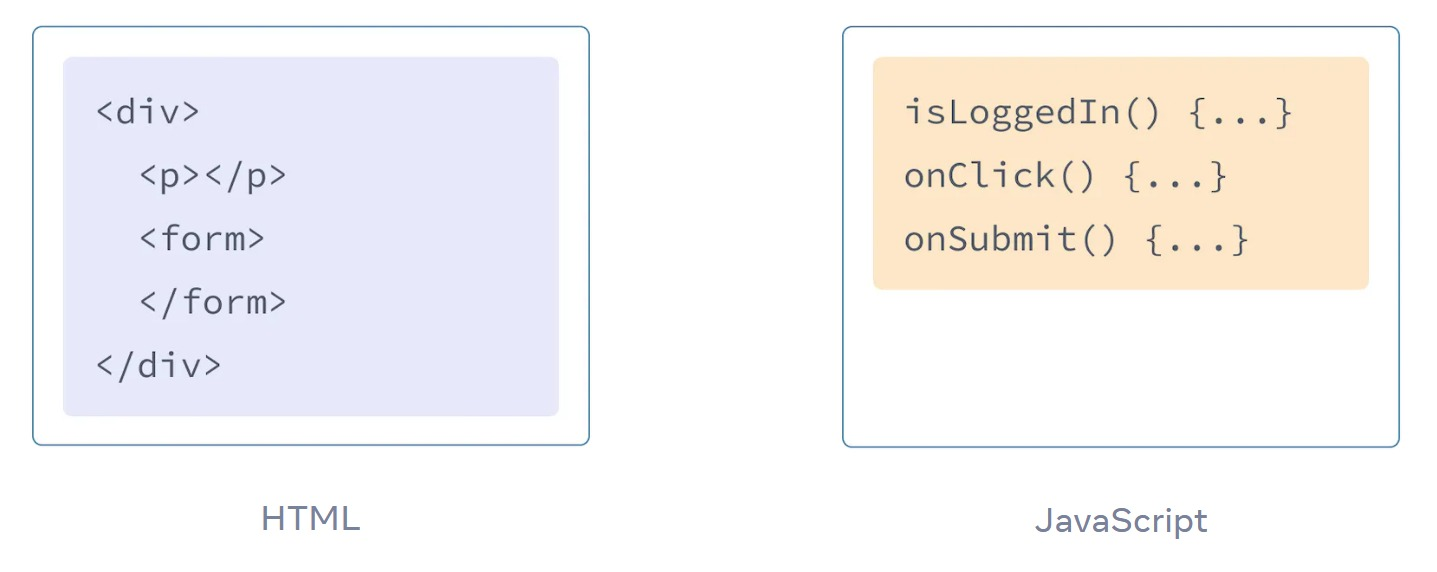
\includegraphics[width=1\textwidth]{images/02/ReactJS-JSX.jpeg}
    \caption{Einfache Grafik von Darstellung und Logik bei Webseiten\cite{react-jsx-html, react-jsx-javascript}}
\end{figure}

Doch aufgrund der zunehmenden Interaktivität und der wachsenden Größe von Webseiten wird heutzutage vermehrt JavaScript und weniger \acs{HTML} und \acs{CSS} verwendet. Dies hat dazu geführt, dass die Grenzen zwischen Logik und Darstellung verschwimmen. Dadurch ist die Trennung zwischen Logik und Darstellung in \acs{JSX} nicht mehr so klar auseinanderzusetzen. Wie in der folgenden Grafik vereinfacht dargestellt:

\begin{figure}[h]
    \centering
    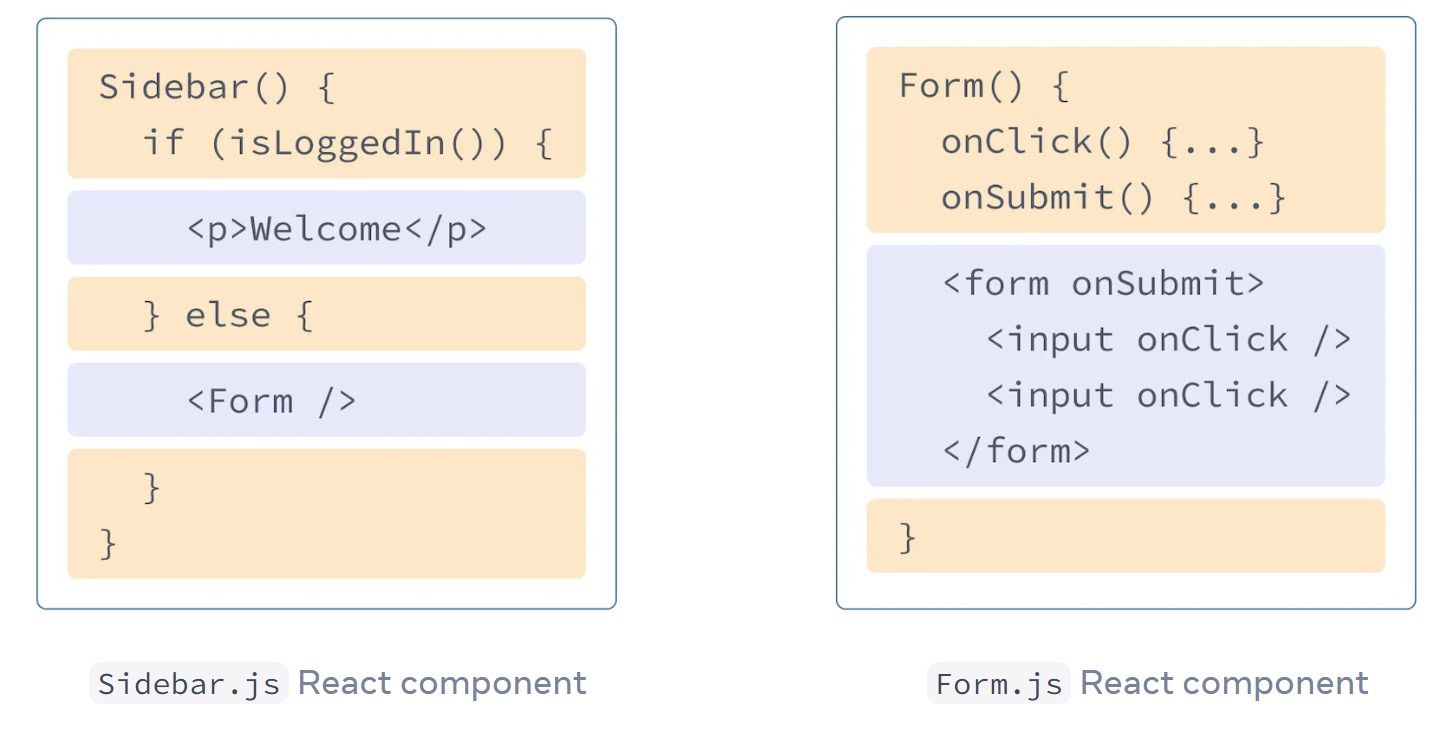
\includegraphics[width=1\textwidth]{images/02/ReactJS-JSX-Component.jpeg}
    \caption{JSX Grafik von Darstellung und Logikverschmelzung\cite{react-jsx-form-component, react-jsx-sidebar-component}}
\end{figure}

Dadurch kann die Darstellung und Logik von zusammenhängenden Komponenten beieinander sein, erhöht das die Möglichkeit, dass der Code aktuell bleibt, und Code oder Komponenten, die wiederum nichts miteinander zu tun haben, sind separiert durch verschiedene JavaScript-Dateien. Somit können EntwicklerInnen besser strukturierten Code schreiben, der sowohl die Logik als auch die Darstellung umfasst. Dieser Ansatz bietet eine nahtlose Integration von JavaScript-Funktionalitäten in die Gestaltung von Benutzeroberflächen. Anstatt verschiedene Dateien für \acs{HTML}, \acs{CSS} und JavaScript zu haben, ermöglicht \acs{JSX} das Verfassen von Komponenten, die sowohl Struktur als auch Verhalten vereinen. Dadurch entsteht eine vereinfachte, effizientere Entwicklung von Webanwendungen.

Die Einführung von \acs{JSX} hat die Art und Weise, wie Webentwicklung betrieben wird, maßgeblich verändert, und sie spielt eine bedeutende Rolle in Frameworks wie \textbf{React.js}, \textbf{Vue} und anderen modernen Bibliotheken zur Entwicklung von Benutzeroberflächen. Diese Entwicklung hat dazu geführt, dass EntwicklerInnen leistungsstarke, interaktive Webanwendungen schneller und effektiver erstellen können.\cite{react-jsx-explained}

\subsection{TypeScript superset JavaScript}

\acf{TS} ist eine von Microsoft entwickelte Programmiersprache, die eine typisierte Erweiterung von \acl{JS} darstellt. Es fügt statische Typen hinzu, was die Code-Qualität verbessert und EntwicklerInnenn ermöglicht, robustere und wartbarere Software zu erstellen. \cite{typescript}

\subsubsection{Schlüsselmerkmale von TypeScript}

\begin{enumerate}
    \item \textbf{Statische Typisierung:} \acl{TS} fügt statische Typisierung hinzu, die es EntwicklerInnenn ermöglicht, Typen für Variablen, Parameter und Rückgabetypen von Funktionen festzulegen. Dies hilft, Fehler frühzeitig im Entwicklungsprozess zu erkennen.

    \item \textbf{Verbesserte Code-Intelligenz:} Durch die Verwendung von \acl{TS} profitiert man von besserer Code-Intelligenz in Entwicklungsumgebungen, was die Produktivität steigert. Intelligente Autovervollständigung und detaillierte Fehlermeldungen sind einige der Vorteile.

    \item \textbf{Interfaces und Typen:} \acl{TS} ermöglicht die Definition von benutzerdefinierten Typen und Schnittstellen, was zu einer klaren und strukturierten Codebasis führt. Dies erleichtert die Zusammenarbeit im Team und das Verständnis des Codes.

    \item \textbf{ES6-Unterstützung:} \acl{TS} unterstützt ECMAScript 6 und darüber hinaus, was bedeutet, dass EntwicklerInnen die neuesten Funktionen von JavaScript nutzen können.

    \item \textbf{Bessere Wartbarkeit und Skalierbarkeit:} Die Verwendung von Typen trägt dazu bei, Bugs zu reduzieren und die Wartbarkeit von Codebasen zu verbessern. Dies ist besonders wichtig für größere Projekte.
\end{enumerate}

\subsection{Moderne Frontend-Frameworks}
\label{chapter:3-frontend-frameworks}

Die Entwicklung von Webanwendungen hat sich in den letzten Jahren stark weiterentwickelt, und moderne Frontend-Frameworks spielen dabei eine entscheidende Rolle. Diese Frameworks erleichtern nicht nur die Erstellung von ansprechenden und interaktiven Benutzeroberflächen, sondern bieten auch viele Funktionen und Werkzeuge, die die Entwicklung effizienter und produktiver machen.

\begin{itemize}

    \item \textbf{Angular:} Angular ist ein von Google entwickeltes \acl{TS}-basierendes Framework. Es bietet eine umfangreiche Sammlung von Werkzeugen und Bibliotheken, die EntwicklerInnenn helfen, dynamische \acf{SPA} zu erstellen. Die Struktur von Angular erleichtert die Organisation des Codes und bietet eine klare Trennung von Logik und Darstellung.\cite{angular}

    \item \textbf{Vue:} Vue.js ist ein progressives \acl{JS}-Framework, das sich durch seine leichte Integration, Flexibilität und eine sanfte Lernkurve auszeichnet. Es ermöglicht die Erstellung interaktiver Benutzeroberflächen und wird von einer aktiven Community unterstützt, die ständig zur Weiterentwicklung und Verbesserung beiträgt.\cite{vuejs}

    \item \textbf{React.js:} React.js, entwickelt von Facebook, ist eine beliebte \acl{JS}-Bibliothek, die sich auf die Erstellung wiederverwendbarer \acf{UI}-Komponenten konzentriert. Durch die Verwendung von \acf{JSX} können EntwicklerInnen eine hierarchische Struktur aufbauen, die zur Erstellung dynamischer Benutzeroberflächen beiträgt.\cite{reactjs}
\end{itemize}

\begin{longtable}{@{\extracolsep{\fill}}|l|l|l|l|@{}}
    \hline
    \multicolumn{1}{|l|}{\textbf{Parameter}} &
    \multicolumn{1}{l|}{\textbf{Angular}}    &
    \multicolumn{1}{l|}{\textbf{React.js}}   &
    \multicolumn{1}{l|}{\textbf{Vue}}                                                                                               \\ \hline
    \endfirsthead
    \hline
    \multicolumn{1}{|l|}{\textbf{Parameter}} &
    \multicolumn{1}{l|}{\textbf{Angular}}    &
    \multicolumn{1}{l|}{\textbf{React.js}}   &
    \multicolumn{1}{l|}{\textbf{Vue}}                                                                                               \\ \hline
    \endhead

    \hline
    \multicolumn{4}{|r|}{{Die Fortsetzung erfolgt auf der nachfolgenden Seite}}                                                     \\ \hline
    \endfoot


    \endlastfoot
    Unterstützung                            & Google     & Facebook     & Community                                                \\ \hline
    Typ                                      & Framework  & Bibliothek   & Framework                                                \\ \hline
    Größe                                    & Mittel     & Klein        & Sehr klein                                               \\ \hline
    Sprache                                  & TypeScript & JavaScript   & JavaScript                                               \\ \hline
    Leistung                                 & Gut        & Gut          & Gut                                                      \\ \hline
    Datenbindung                             & Beide      & Einfach      & Einfach                                                  \\ \hline
    Lernkurve                                & Steil      & Einfach      & Einfach                                                  \\ \hline
    Nutzung                                  & 2.         & 1.           & 3.                                                       \\ \hline
    Entwicklungsgeschwindigkeit              & Mittel     & Relativ kurz & Schnell                                                  \\ \hline
    Am besten geeignet für                   & PWA, SPA   & E-Commerce   & Schnelle Entwicklung                                     \\ \hline
    \caption{Vergleich von Angular, Vue und React.js \cite{angular-vuejs-reactjs-comparison:1, angular-vuejs-reactjs-comparison:2}} \\
\end{longtable}

Diese Frameworks haben jeweils ihre eigenen Stärken und eignen sich für unterschiedliche Projekte je nach Anforderungen, Teampräferenzen und Zielen.\cite{angular-vuejs-reactjs-comparison:3, angular-vuejs-reactjs-comparison:4}
Bei allen Frameworks steht eine Frontendtechnologie besonders im Vordergrund: Single-Page-Applications (\acs{SPA}).
Eine \acs{SPA} hat den Hintergedanken, dass die gesamte Anwendung auf nur einer Webseite dargstellt wird und läuft. \cite*{spa}
Bei einer \acs{SPA} wird die gesamte Präsentationsschicht vom Browser durchgeführt.
Dabei übernimmt der Client bzw. der Browser die Aufgabe, \acs{HTML}-Code und Daten zu vereinen. \cite{spa}
Man kann sich das ganze in folgendem Beispiel vorstellen:\\
Eine NutzerIn hat eine Webseite vor Augen. Auf der Webseite ist ein Button, der beim Drücken Daten anfordert und diese auf einer Webseite anzeigen soll.
Anstatt die Daten von einem Server zu holen, auf einer Seite einzubauen und die gesamte Webseite neu zu laden, nutzen \acs{SPA}'s dynamisches Rendering.
Es wird also vereinfacht gesagt, platz auf der bereits vorhandenen Webseite gemacht, um den neuen Inhalt (die Daten) dynamisch ohne alles neu zu laden, anzuzeigen.
Die NutzerIn merkt aufgrund des dynamischen Einfügens häufig gar nicht, dass im Hintergrund etwas passiert.
Dieses Vorgehen nennt man in der Fachsprache auch \textbf{clientseitiges Rendering}.

Die CO2-Runter-App wurde ursprünglich mit \textbf{React.js} entwickelt. Allerdings fiel die Entscheidung, das Framework zu wechseln, da die EntwicklerInnen mit \textbf{React.js} nicht zufrieden waren und auf diverse Probleme stießen. Als Alternative wurde \textbf{Vue} ausgewählt, da es eine leicht verständliche Lernkurve aufweist und die EntwicklerInnen bereits Erfahrung damit hatten. Zudem zeichnet sich \textbf{Vue} durch hohe Flexibilität aus und lässt sich gut mit anderen Bibliotheken und Frameworks kombinieren. Die Entscheidung für \textbf{Vue} wurde auch durch seine Performance und umfassende Dokumentation beeinflusst, was die Entwicklung erleichtert.

\section{Werkzeuge}
\label{chapter:3-werkzeuge}

Bei der Weiterentwicklung der CO2-Runter-App kommen zahlreiche Tools zum Einsatz, um die Entwicklungsumgebung zu verbessern und die Entwicklung zu vereinfachen. Da jedoch einige Tools auf das Backend und die Datenbank bezogen sind, werden diese hier außen vor gelassen. Es wird ausschließlich auf diejenigen eingegangen, die für die Frontend-Entwicklung relevant sind. Diese Tools sind wichtig für die Weiterentwicklung der CO2-Runter-App und spielen auch für das nutzerzentrierte Design eine Rolle.

\subsection{NPM - Node Package Manager}
\label{chapter:3-werkzeuge-npm}

\acs{NPM} ist die Abkürzung für \acf{NPM}. Wie der Name schon sagt, ist NPM ein Paketmanager, der bei der Installation von Node.js mitgeliefert wird. Er ermöglicht somit die Installation und Verwaltung von JavaScript-Paketen.

Ein Paketmanager ist eine Software, die es ermöglicht, sogenannte Pakete herunterzuladen und in ein Projekt zu importieren. Unter einem Paket versteht man ein Projekt, das von EntwicklerInnen bereitgestellt wurde, um von anderen EntwicklerInnenn in deren Projekten eingebunden zu werden. Auf diese Weise können EntwicklerInnen ihre Arbeit miteinander teilen und Zeit sparen, indem sie bereits vorhandene Projekte verwenden, anstatt alles von Grund auf neu entwickeln zu müssen.

Für jeden Paketmanager gibt es eine Paketzentrale oder auch Registry genannt. In der Registry von \acs{NPM} sind über 800.000 Pakete/Projekte zu finden. \acs{NPM} ermöglicht außerdem, eine bestimmte Version eines Pakets in ein Projekt zu importieren. Diese Funktion erlaubt es EntwicklerInnen, selbst mit veralteten Versionen eines Projekts weiterzuarbeiten. \acs{NPM} ist nur einer von vielen Paketmanagern, die es gibt, dennoch hat sich \acs{NPM} im JavaScript-Umfeld als das Standardwerkzeug für die Paketverwaltung herausgebildet.\cite{npm}

\subsection{Vite}

Vite ist ein modernes Build-Tool, das speziell für die Entwicklung von Webanwendungen mit modernen Technologien wie Vue, React und TypeScript entwickelt wurde. Es wurde entworfen, um die Entwicklung zu beschleunigen, indem es schnelle Builds und eine effiziente Entwicklungsumgebung bereitstellt. \cite{vitejs}

\subsubsection{Merkmale von Vite}

\begin{enumerate}
    \item \textbf{Schnelle Entwicklungsumgebung:} Vite bietet eine extrem schnelle Entwicklungszeit, indem es eine schnelle Startzeit und inkrementelle Builds ermöglicht. Dies erleichtert die Entwicklung und Tests während des Schreibens von Code.

    \item \textbf{Effizientes HMR (Hot Module Replacement):} Mit HMR können Änderungen im Code sofort angewendet werden, ohne dass die gesamte Anwendung neu geladen werden muss. Dies beschleunigt den Entwicklungsprozess erheblich.

    \item \textbf{Unterstützung für verschiedene Frameworks:} Vite unterstützt verschiedene Frontend-Frameworks wie Vue, React und sogar Vanilla JavaScript, was es flexibel für verschiedene Projekte macht.

    \item \textbf{Eingebautes Dev-Server:} Der integrierte Entwicklungsserver von Vite bietet eine optimale Erfahrung während der Entwicklung, einschließlich Fehlermeldungen im Browser, automatischem Öffnen des Browsers und mehr.

    \item \textbf{Effizientes Bundling:} Vite nutzt ESM (ECMAScript Module) und bietet ein effizientes Bundling für die Produktion, was zu kleinen und schnellen Build-Dateien führt.
\end{enumerate}

\subsection{Material Design Bibliothek}

Material Design ist ein Designsystem, das von Google entwickelt wurde, um eine konsistente und ansprechende Benutzeroberfläche für Web- und Mobilanwendungen zu schaffen. Es basiert auf den Prinzipien von Material Design, die auf visueller Hierarchie, Bewegung und Interaktion basieren. Material Design bietet eine Reihe von Komponenten, Icons und Stilen, die EntwicklerInnenn helfen, moderne und benutzerfreundliche Benutzeroberflächen zu erstellen. \cite{materialdesign}

Da Material Design Richtlinien von Google sind, entwickeln Dritte Bibliotheken, die diese Richtlinien umsetzen. Dabei gibt es jeweils Bibliotheken für die unterschiedlichen Frontend-Frameworks. Für Vue gibt es z. B. Vuetify, für React gibt es Material-UI und für Angular gibt es Angular Material. Da die vorherige CO2-Runter-App auf React.js basierte, wurde dort die Material-UI Bibliothek verwendet. Um ein äquivalentes Design zu erreichen, wird in der Weiterentwicklung der CO2-Runter-App die Vuetify-Bibliothek verwendet, die speziell für Vue.js entwickelt wurde, aber dennoch die Material Design Richtlinien von Google umsetzt, wie auch die Material-UI (MUI) Bibliothek.

Beide Bibliotheken bieten eine Vielzahl von Komponenten, zum Beispiel Knöpfe, Textfelder etc., die EntwicklerInnen ermöglichen, schnell und einfach eine schöne und moderne Benutzeroberfläche zu erstellen. \acf{MUI} oder auch Vuetify sind dabei \acs{UI}-Komponenten-Bibliotheken, die auf React.js oder Vue basieren und die Material Design Richtlinien von Google anwenden, um ein einheitliches, schönes modulares Design zu schaffen, und somit die Entwicklung von Webanwendungen oder Prototypen zu vereinfachen.\cite{materialui, vuetify}

\subsection{NGINX}

Für die Entwicklung von Webanwendungen ist ein Webserver unerlässlich. \acf{NGINX} ist ein Open-Source-Webserver, der für seine Leistung, Skalierbarkeit und Zuverlässigkeit bekannt ist. Er wird häufig als Reverse-Proxy-Server, Lastausgleichs-Server und HTTP-Cache verwendet. \acs{NGINX} bietet eine Vielzahl von Funktionen, die es zu einem beliebten Webserver für die Entwicklung und Bereitstellung von Webanwendungen machen.

\acs{NGINX} fungiert als Reverse-Proxy-Server, der eingehende Anfragen an verschiedene Backend-Server weiterleitet. Diese Funktion ermöglicht eine flexible Konfiguration von Routen und eine effiziente Verteilung des Datenverkehrs. Zum Beispiel kann \acs{NGINX} den Datenverkehr basierend auf bestimmten Kriterien wie IP-Adresse, Header oder URL auf verschiedene Backend-Server verteilen. Dadurch können Anwendungen skalierbarer gestaltet werden, da \acs{NGINX} den Datenverkehr je nach Bedarf auf zusätzliche Server umleiten kann, um die Last zu verteilen und die Ausfallsicherheit zu erhöhen.

Ein weiterer wichtiger Aspekt von \acs{NGINX} ist sein HTTP-Caching. Durch den Einsatz von \acs{NGINX} als HTTP-Cache können statische Inhalte wie Bilder, CSS-Dateien und JavaScript-Dateien zwischengespeichert werden. Dies reduziert die Last auf Backend-Servern und beschleunigt die Ladezeiten für BenutzerInnen, da häufig angeforderte Ressourcen direkt aus dem Cache bereitgestellt werden können. Darüber hinaus kann \acs{NGINX} auch als Reverse-Proxy-Cache dienen, indem es die Antworten von Backend-Servern zwischenspeichert, um wiederholte Anfragen zu beschleunigen und die Serverlast zu verringern.

\acs{NGINX} ermöglicht es uns, die Datenbank, die \acs{API} und das Frontend zu verbinden. Es ist ein wichtiger Bestandteil der Infrastruktur, da es die Kommunikation zwischen den verschiedenen Komponenten der Anwendung ermöglicht. \acs{NGINX} bietet eine leistungsstarke und flexible Plattform für die Bereitstellung von Webanwendungen und ist ein unverzichtbares Werkzeug für die Entwicklung und Bereitstellung von modernen Webanwendungen. \cite{nginx}

\subsection{Docker}

Docker ist eine Open-Source-Plattform, die es EntwicklerInnenn ermöglicht, Anwendungen in Containern zu erstellen, zu testen und zu bereitstellen. Container sind eine Art von Virtualisierung, die es ermöglichen, Anwendungen und ihre Abhängigkeiten in einer isolierten Umgebung auszuführen. Docker bietet eine Vielzahl von Funktionen, die die Entwicklung und Bereitstellung von Anwendungen erleichtern, darunter die Möglichkeit, Anwendungen in Containern zu verpacken, Container zu verwalten und Container in der Cloud zu bereitstellen.

Eine der leistungsstarken Funktionen von Docker ist die Möglichkeit, Anwendungen über verschiedene Umgebungen hinweg zu skalieren und bereitzustellen. Durch die Verwendung von Docker-Containern können EntwicklerInnen sicherstellen, dass ihre Anwendungen konsistent und deterministisch in verschiedenen Umgebungen ausgeführt werden, von lokalen Entwicklungsumgebungen bis hin zu Produktionsumgebungen in der Cloud.

Darüber hinaus bietet Docker eine einfache Möglichkeit, Anwendungen horizontal zu skalieren, indem mehrere Instanzen von Containern gestartet und verwaltet werden können. Dies ermöglicht eine effiziente Nutzung von Ressourcen und verbessert die Skalierbarkeit von Anwendungen, insbesondere in hoch belasteten Umgebungen.

Ein weiterer Vorteil von Docker ist die Portabilität von Containern. Docker-Container können leicht zwischen verschiedenen Umgebungen verschoben werden, da sie alle ihre Abhängigkeiten und Konfigurationen in einem Paket enthalten. Dies erleichtert die Bereitstellung von Anwendungen auf verschiedenen Infrastrukturen, von lokalen Rechnern bis hin zu öffentlichen Cloud-Plattformen wie AWS, Azure oder Google Cloud.

Docker ermöglicht es uns, die Anwendung in einer isolierten Umgebung zu testen und zu entwickeln, ohne dass die Umgebung der EntwicklerInnen beeinträchtigt wird. Es bietet eine konsistente und zuverlässige Plattform für die Entwicklung und Bereitstellung von Anwendungen und ist ein unverzichtbares Werkzeug für die Entwicklung moderner Webanwendungen. \cite{docker}

% Überleitung ins nächste Kapitel

Nachdem die Grundlagen der nutzerzentrierten Design-Methoden und der Webentwicklung erläutert wurden, wird im nächsten Kapitel auf die Nutzerzentrierte Umfrage eingegangen. Im folgenden Kapitel wird beschrieben, wie eine nutzerzentrierte Umfrage aufgebaut wird und welche verschiedenen Arten einer Umfrage es gibt. Anschließend wird erläutert, welche Faktoren bei der Auswahl der Zielgruppe entscheidend sind und wie die tatsächliche Durchführung der nutzerzentrierten Umfrage verlief. Es werden die Ergebnisse der im Rahmen dieser Studienarbeit durchgeführten Umfrage offengelegt und analysiert. Abschließend wird das Thema Personas angesprochen.
